% Created 2015-11-15 Sun 18:26
\documentclass[9pt]{beamer}
\usepackage[utf8]{inputenc}
\usepackage[T1]{fontenc}
\usepackage{fixltx2e}
\usepackage{graphicx}
\usepackage{longtable}
\usepackage{float}
\usepackage{wrapfig}
\usepackage{soul}
\usepackage{textcomp}
\usepackage{marvosym}
\usepackage{wasysym}
\usepackage{latexsym}
\usepackage{amssymb}
\usepackage{hyperref}
\tolerance=1000
\mode<beamer>{\usetheme{Warsaw}}
\mode<beamer>{\setbeamertemplate{blocks}[rounded][shadow=false]}
\mode<beamer>{\addtobeamertemplate{block begin}{\pgfsetfillopacity{0.8}}{\pgfsetfillopacity{1}}}
\mode<beamer>{\setbeamercolor{structure}{fg=orange}}
\mode<beamer>{\setbeamercovered{transparent}}
\AtBeginSection[]{\begin{frame}<beamer>\frametitle{Topic}\tableofcontents[currentsection]\end{frame}}
\usepackage{subcaption}
\usepackage{multimedia}
\usepackage{tikz}
\usepackage{subfigure,subfigmat}
\usepackage{threeparttable}
\usetikzlibrary{shapes,arrows,shadows}
\usepackage{bm, amssymb, amsmath, array, pdfpages,graphicx}
\newcommand{\bv}[1]{\mathbf{#1}}
\newcommand{\diff}[2]{\frac{\partial #1}{\partial #2}}
\newcommand{\beq}[0]{\begin{equation}}
\newcommand{\eeq}[0]{\end{equation}}
\newcommand{\beqa}[0]{\begin{eqnarray}}
\newcommand{\eeqa}[0]{\end{eqnarray}}
\newcommand{\beqq}[0]{\begin{equation*}}
\newcommand{\eeqq}[0]{\end{equation*}}
\newcommand{\bs}[1]{\boldsymbol{#1}}
\newcommand{\ip}[2]{\langle #1, #2\rangle}
\providecommand{\alert}[1]{\textbf{#1}}

\title{Uncertainty Quantification of Low-Dimensional Models}
\author{Anthony DeGennaro \newline Scott Dawson \newline Clarence W. Rowley III \newline Princeton University}
\date{APS 68$^{th}$ Annual DFD Meeting \\ Boston, MA \\ November 2015}
\hypersetup{
  pdfkeywords={},
  pdfsubject={},
  pdfcreator={Emacs Org-mode version 7.9.3f}}

\begin{document}

\maketitle

\begin{frame}
\frametitle{Outline}
\setcounter{tocdepth}{3}
\tableofcontents
\end{frame}



% Define my settings

\graphicspath{{../Figures/}}
% Add Princeton shield logo
\addtobeamertemplate{frametitle}{}{%
\begin{tikzpicture}[remember picture,overlay]
\node[anchor=north east,yshift=2pt] at (current page.north east) {\includegraphics[height=0.7cm]{Shield}};
\end{tikzpicture}}
%


\institute{Princeton University}


\section{Introduction}
\label{sec-1}
\begin{frame}
\frametitle{Motivation}
\label{sec-1-1}

\begin{itemize}
\item Low-dimensional modeling is a useful method for examining high-dimensional data
\begin{itemize}
\item Proper Orthogonal Decomposition (POD)
\begin{itemize}
\item Data compression
\item Dominant spatial features
\item Inexpensive models
\end{itemize}
\item Dynamic Mode Decomposition (DMD)
\begin{itemize}
\item Linear description of dynamical system
\item Spatial modes + frequencies
\end{itemize}
\end{itemize}
\item Uncertainty quantification is a useful method for investigating statistical variations
\begin{itemize}
\item Polynomial Chaos Expansions (PCE)
\begin{itemize}
\item Assumes \emph{a-priori} probabilistic knowledge of uncertainty
\item Efficient sampling algorithm
\item Accurate surrogate model
\end{itemize}
\end{itemize}
\item \textbf{Can we investigate statistical variations in low-dimensional models efficiently/accurately?}
\end{itemize}
\end{frame}
\begin{frame}
\frametitle{Applications}
\label{sec-1-2}

\begin{itemize}
\item POD Galerkin Models of Fluid Flows
\begin{itemize}
\item Computationally-inexpensive model
\begin{itemize}
\item Collect data from simulations/experiments
\item Calculate POD of output data
\item Project governing flow equations onto POD modes
\end{itemize}
\end{itemize}
\item DMD Analysis of Fluid Flows
\begin{itemize}
\item Determine linear modes/frequencies describing flow behavior
\end{itemize}
\item Sensitive to parametric variations/uncertainties
\begin{itemize}
\item Physical parameters (eg. Reynolds number)
\item Boundary conditions
\item Sensor noise
\end{itemize}
\end{itemize}
\end{frame}
\section{Methodology}
\label{sec-2}
\begin{frame}
\frametitle{Methodology}
\label{sec-2-1}

\begin{itemize}
\item Identify source of uncertainty
\begin{itemize}
\item Physical parameters (eg. Reynolds number)
\item Boundary conditions
\item Sensor noise
\end{itemize}
\item Write a probabilistic description of uncertainty (ie. PDF)
\item Utilize efficient sampling of probability space
\begin{itemize}
\item Quadrature nodes corresponding to a spectral basis
\end{itemize}
\item Collect simulation data using discrete points in probability space
\begin{itemize}
\item Immersed boundary projection method (IBPM) code
\end{itemize}
\item Quantify uncertainty in outputs
\begin{itemize}
\item POD modes
\item DMD modes
\item DMD eigenvalues
\end{itemize}
\end{itemize}
\end{frame}
\begin{frame}
\frametitle{Polynomial Chaos Expansions (PCE)}
\label{sec-2-2}

\begin{itemize}
\item \textbf{Polynomial Chaos Framework} \footnote{Xiu D. \emph{Numerical Methods for Stochastic Computations: A Spectral Method Approach}. Princeton University Press, 2010.
 }
\begin{itemize}
\item Let $\bv{Z} = (Z_1 \ldots Z_d)$ be $d$ random variables with PDF
    $\rho(\bv{Z})$ that parameterize ice
\item Let $\lbrace \Phi_k \rbrace$ denote the set of polynomials
    which are orthogonal w.r.t. $\rho(\bv{Z})$
\item Let $y(\bv{Z})$ denote the mapping from $\bv{Z}$ to an aerodynamic
    performance metric
\end{itemize}
\item \textbf{Probabilistic Collocation Method:}
\begin{itemize}
\item \emph{Representation} 
    \begin{equation*}
      y(\bv{Z}) \approx \sum_{|i|=0}^N y_i \Phi_i(\bv{Z})
    \end{equation*}
\item \emph{Orthonormality} 
    \begin{equation*}
    \begin{aligned}
      \ip{f}{g} &= \int_{\Gamma} f(\bv{z})g(\bv{z}) \rho(\bv{z}) d\bv{z} \\
      \ip{\Phi_i}{\Phi_j} &= \delta_{ij}
    \end{aligned}
    \end{equation*}
\item \emph{Quadrature} 
    \begin{equation*}
      y_k = \ip{y}{\Phi_k} \approx \sum_{i=0}^{Q}
    y(\bv{Z}^{(k)}) \Phi_k(\bv{Z}^{(k)}) w_k
    \end{equation*}
\end{itemize}
\end{itemize}
\end{frame}
\begin{frame}
\frametitle{Polynomial Chaos Expansions (PCE)}
\label{sec-2-3}

\begin{figure}[ht]
\centering
\begin{minipage}[b]{0.45\linewidth}
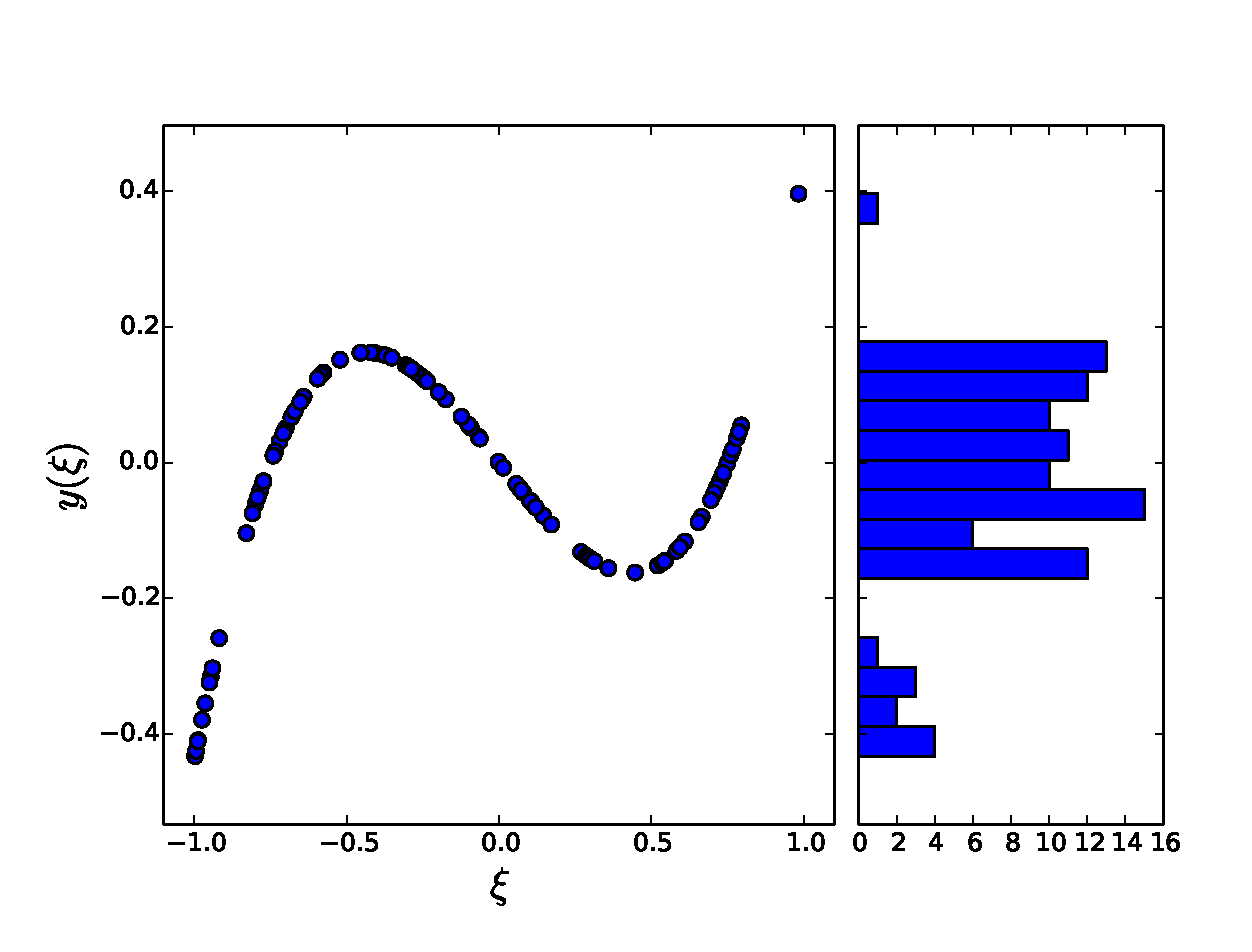
\includegraphics[width=0.9\textwidth]{MCSampling} \\
\centering
\textbf{Monte Carlo} \\
\begin{equation*}
  y \approx \delta(\xi - \xi_k)
\end{equation}
\end{minipage}
\begin{minipage}[b]{0.45\linewidth}
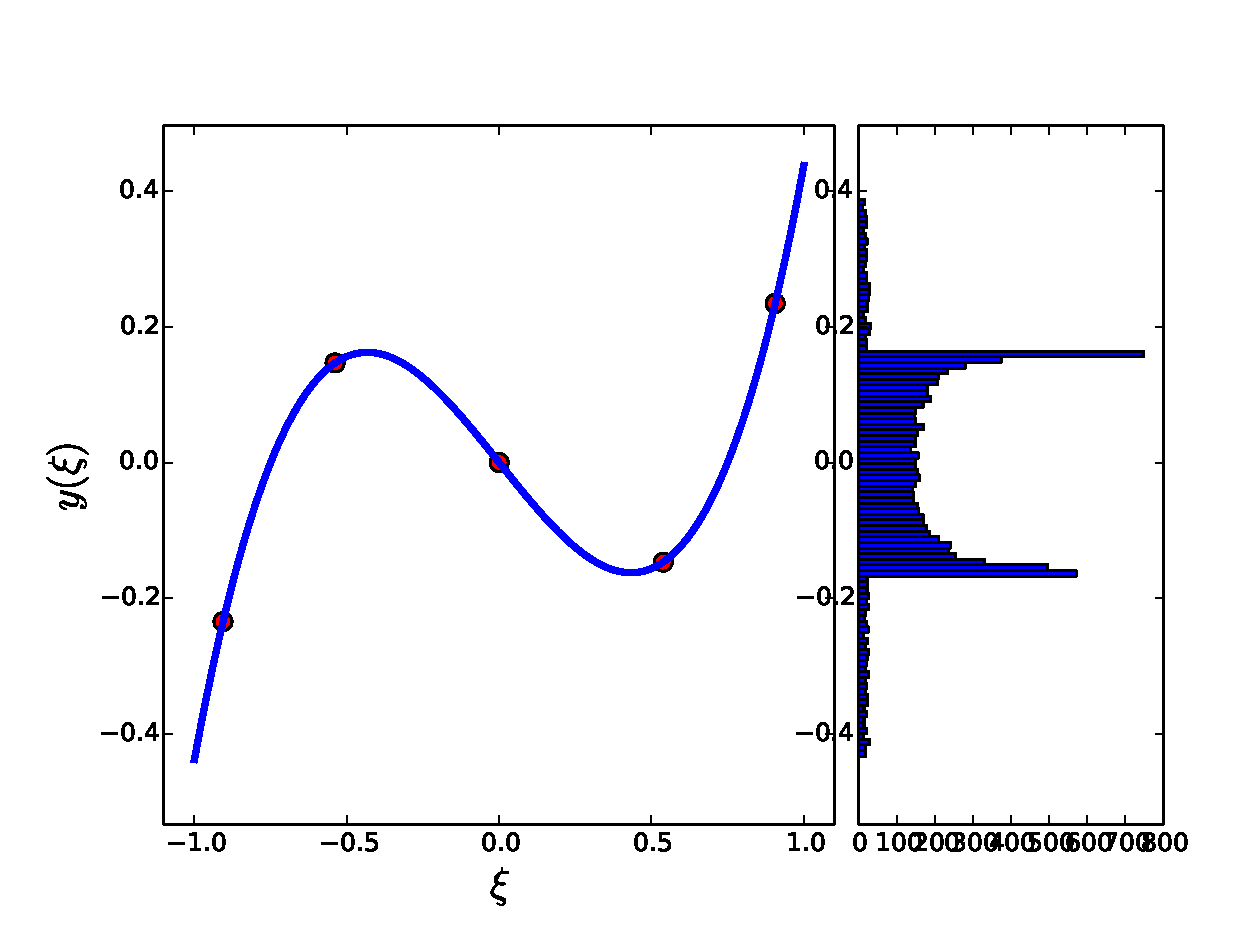
\includegraphics[width=0.9\textwidth]{PCESampling} \\
\centering
\textbf{Polynomial Chaos}
\begin{equation*}
  y \approx \sum_{i}^{Q} c_i \psi_i(\xi)
\end{equation}
\end{minipage}
\end{figure}
\begin{columns}[c]
  \column{0.5\textwidth}
      \begin{itemize}
      \item Draw random samples from distribution
      \item Function exists at discrete points
    \end{itemize}
  \column{0.5\textwidth}
    \begin{itemize}
      \item Use $Q$ quadrature points
      \item Construct $(Q-1)$ order polynomial fit
    \end{itemize}
\end{columns}
\end{frame}
\begin{frame}
\frametitle{Polynomial Chaos Expansions (PCE)}
\label{sec-2-4}

\begin{columns}[c]
  \column{0.5\textwidth}
    \centering
    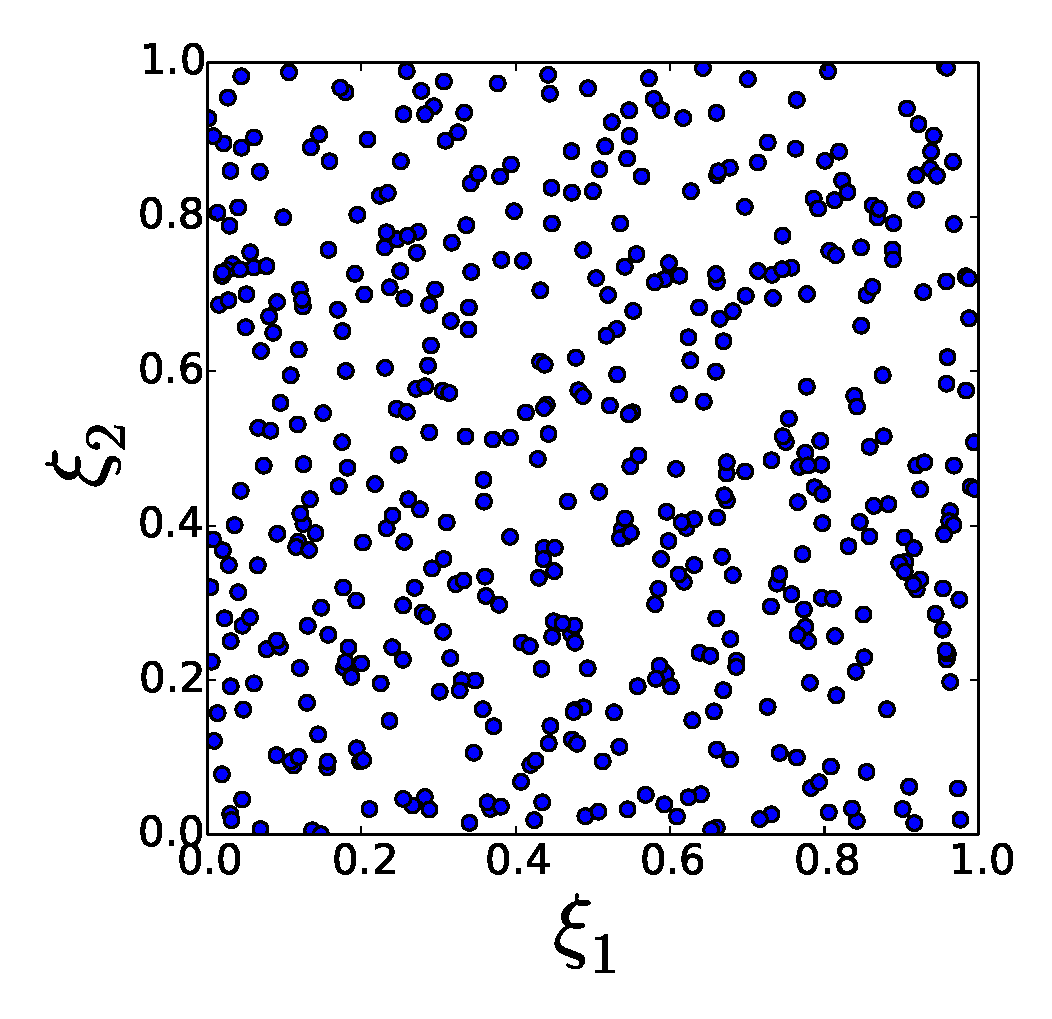
\includegraphics[width=0.9\textwidth]{MonteCarlo} \\
    \bf{Quadrature Sampling Grid}
  \column{0.5\textwidth}
    \centering
    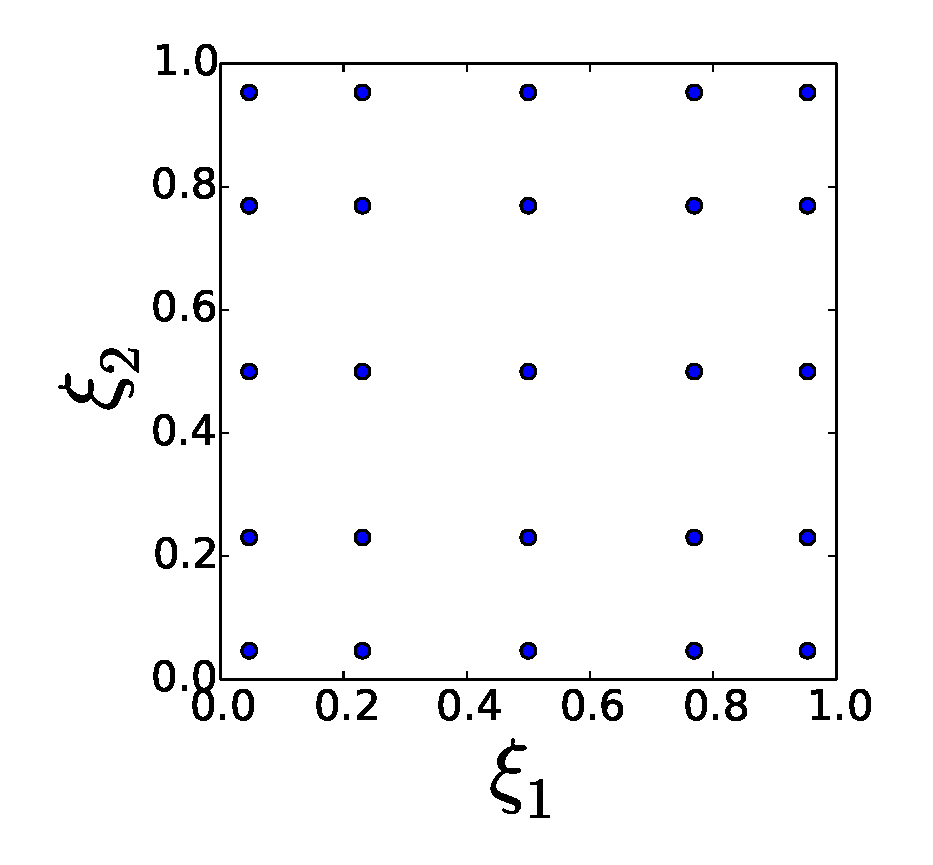
\includegraphics[width=0.9\textwidth]{QuadraturePoints} \\
    {\bf Monte Carlo Sampling}
\end{columns}
\end{frame}
\section{Example: Cylinder Flow POD Modes}
\label{sec-3}
\begin{frame}
\frametitle{Setup}
\label{sec-3-1}

\begin{columns}[c]
\column{0.3\textwidth}
   \centering
    \textbf{Small Spike} \\
    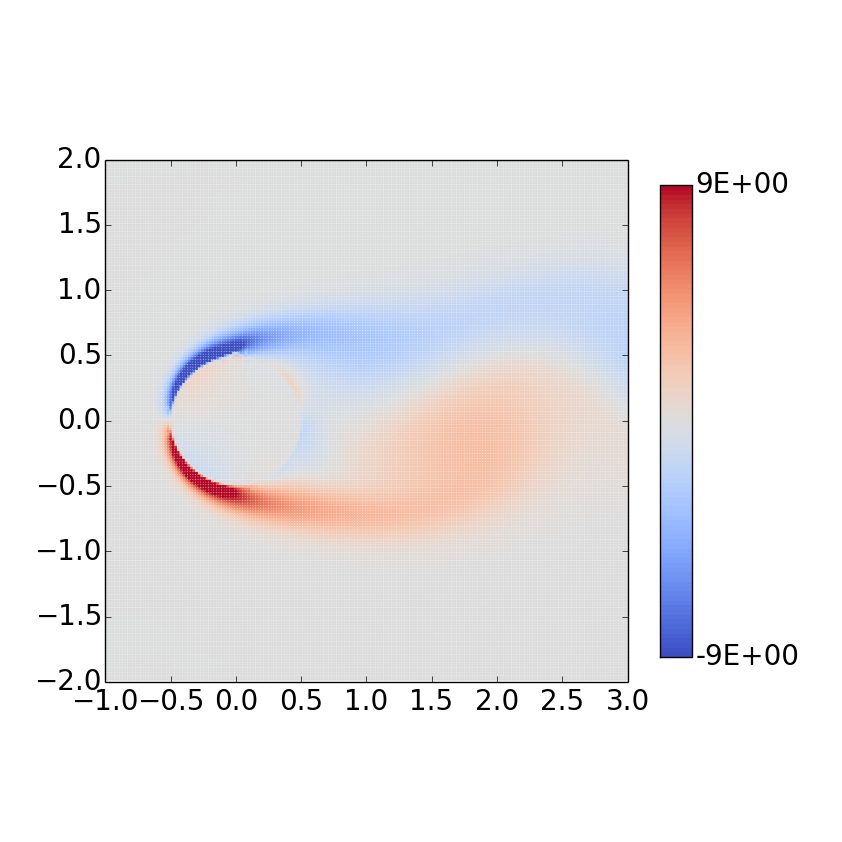
\includegraphics[width=1\textwidth]{PerturbSmallHorn}
\column{0.3\textwidth}
   \centering
    \textbf{Medium Spike} \\
    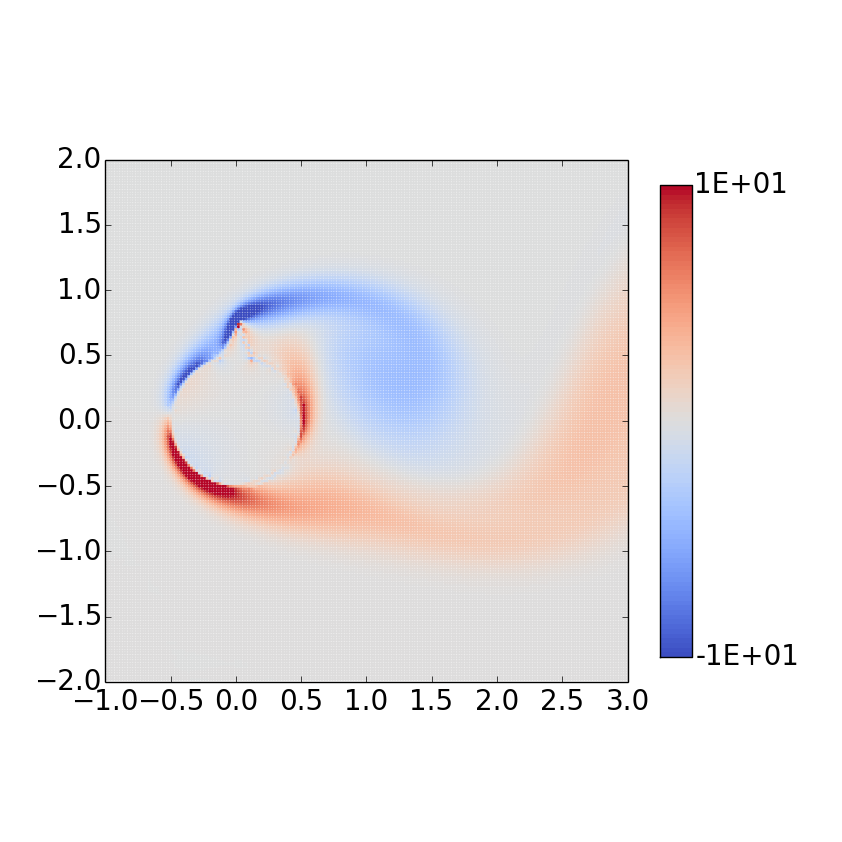
\includegraphics[width=1\textwidth]{PerturbMediumHorn}
\column{0.3\textwidth}
   \centering
    \textbf{Large Spike} \\
    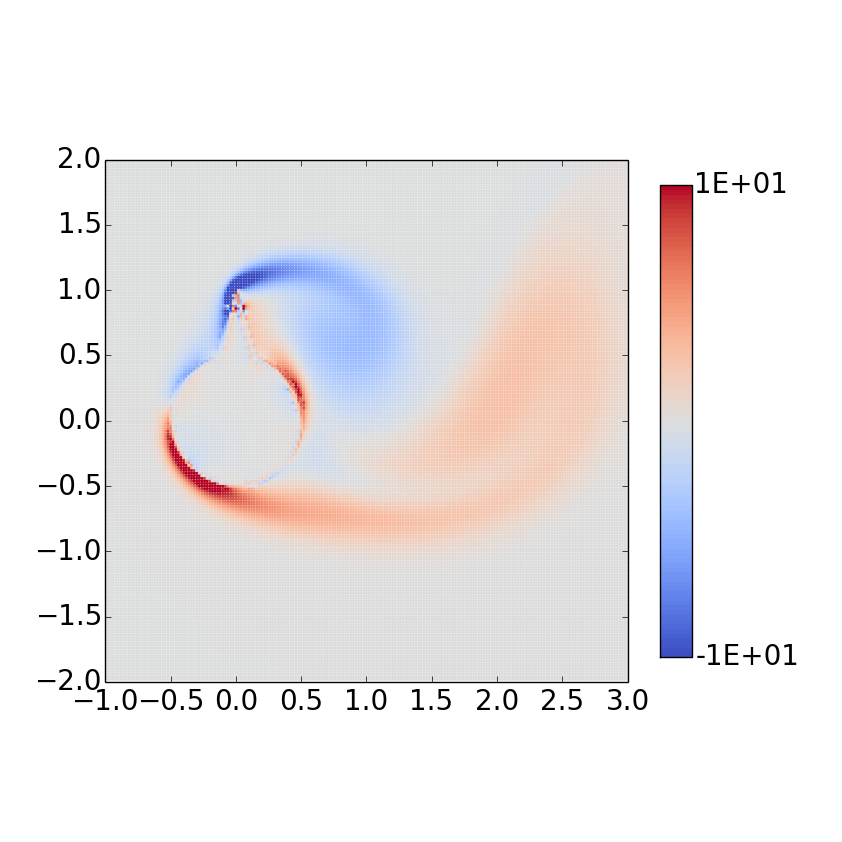
\includegraphics[width=1\textwidth]{PerturbBigHorn}
\end{columns}

\begin{columns}[c]
\column{0.3\textwidth}
   \centering
\column{0.3\textwidth}
   \centering
    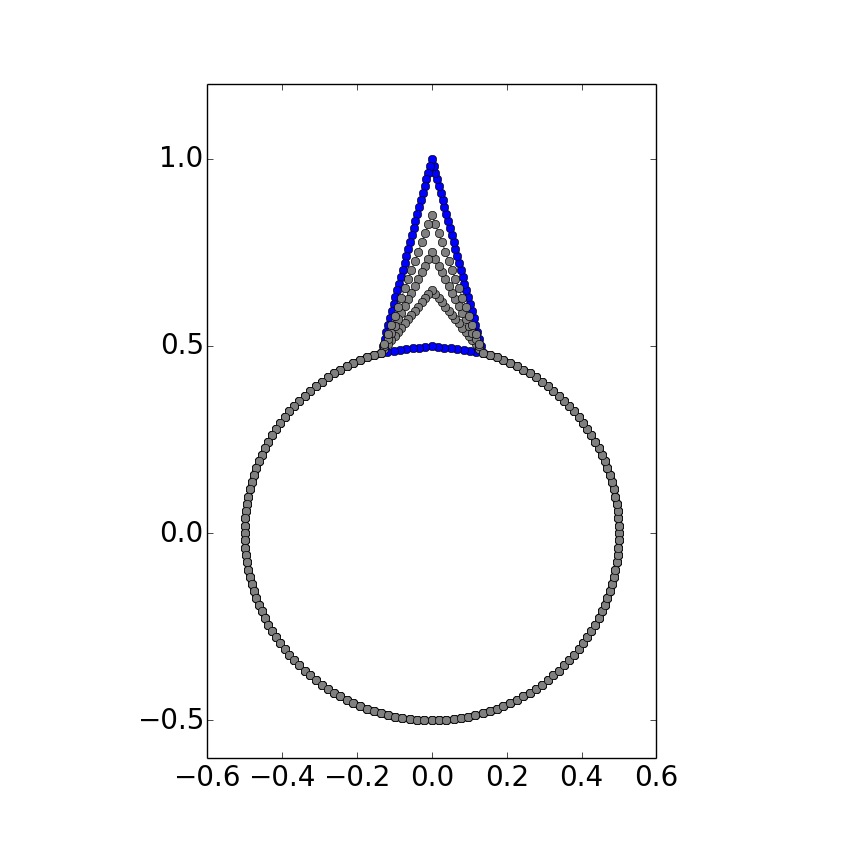
\includegraphics[width=1\textwidth]{CylinderPerturbations}
\column{0.3\textwidth}
   \centering
\end{columns}
\end{frame}
\begin{frame}
\frametitle{Range of Flow Behavior}
\label{sec-3-2}

\begin{columns}[c]
\column{0.5\textwidth}
   \centering
    \textbf{Cylinder, Re = 100}
    \movie[width=0.9\textwidth,height=0.3\textwidth,poster,autostart,loop,borderwidth]{}{CylinderRe100.mp4} \\
    \textbf{POD Modes} \\
    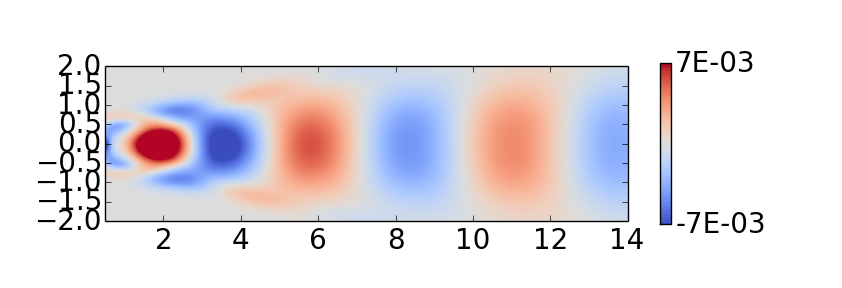
\includegraphics[width=0.9\textwidth]{CylinderRe100POD1} \\
    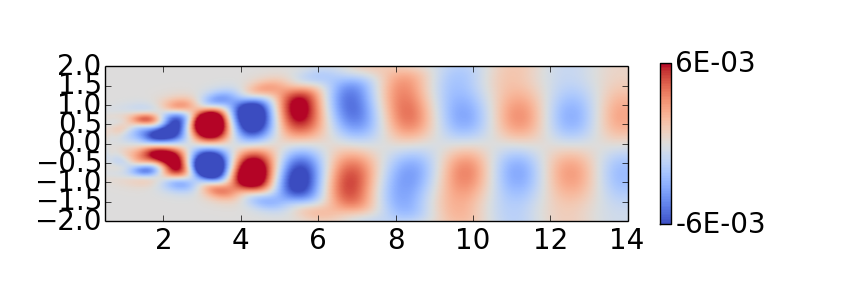
\includegraphics[width=0.9\textwidth]{CylinderRe100POD2} \\
    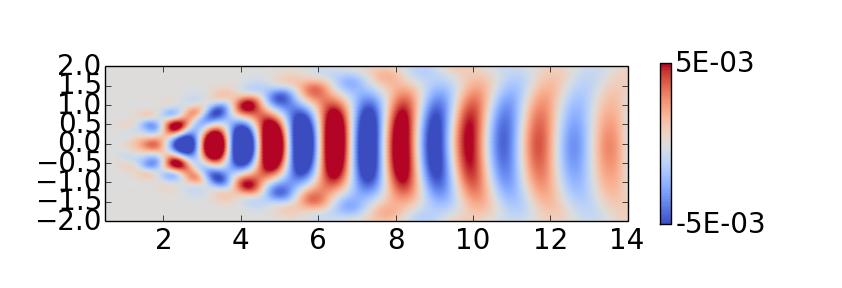
\includegraphics[width=0.9\textwidth]{CylinderRe100POD3}
\column{0.5\textwidth}
   \centering
    \textbf{Perturbed Cylinder, Re = 100}
    \movie[width=0.9\textwidth,height=0.3\textwidth,poster,autostart,loop,borderwidth]{}{PerturbCylinderRe100R1.mp4} \\
    \textbf{POD Modes} \\
    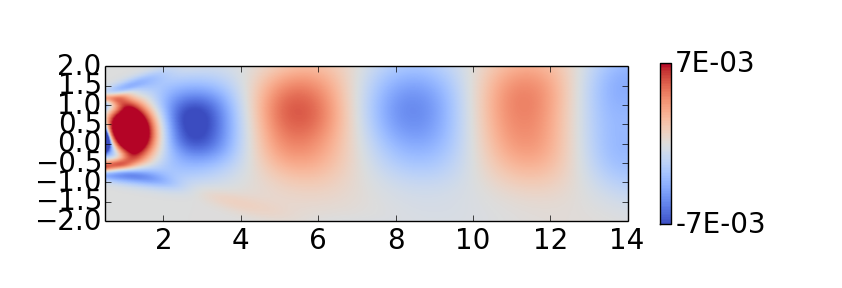
\includegraphics[width=0.9\textwidth]{PerturbRp95Re100POD1} \\
    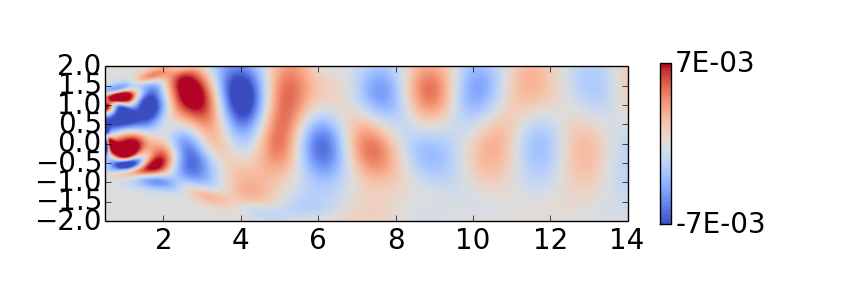
\includegraphics[width=0.9\textwidth]{PerturbRp95Re100POD2} \\
    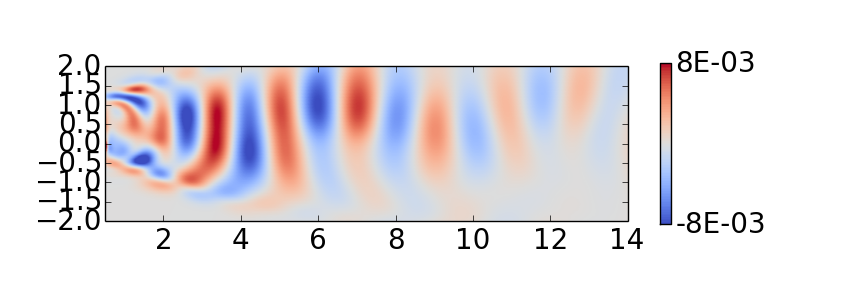
\includegraphics[width=0.9\textwidth]{PerturbRp95Re100POD3}
\end{columns}
\end{frame}
\begin{frame}
\frametitle{Statistical Variance in Modes}
\label{sec-3-3}

\centering
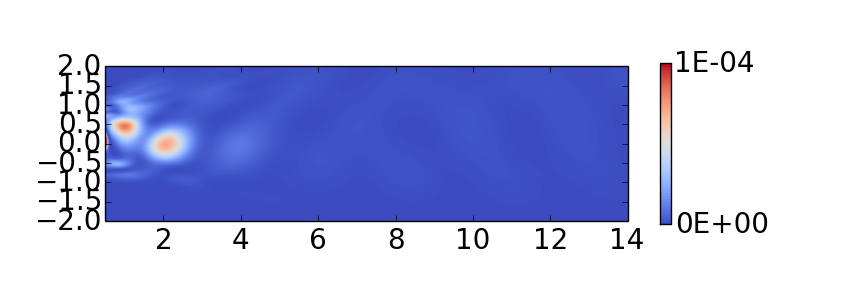
\includegraphics[width=0.5\textwidth]{VariancePOD1} \\
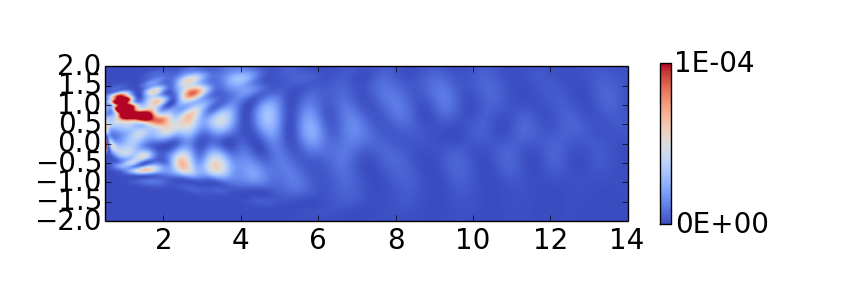
\includegraphics[width=0.5\textwidth]{VariancePOD2} \\
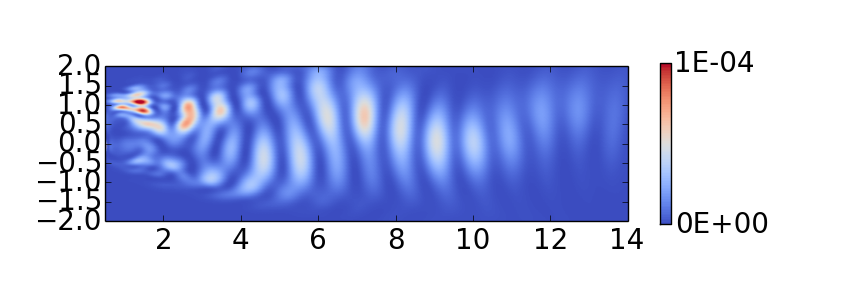
\includegraphics[width=0.5\textwidth]{VariancePOD3} \\
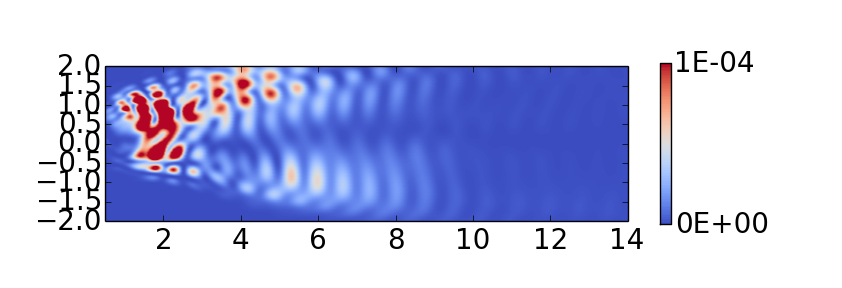
\includegraphics[width=0.5\textwidth]{VariancePOD4} \\
\end{frame}
\begin{frame}
\frametitle{Projection Error}
\label{sec-3-4}

\begin{itemize}
\item Choose the $Q-1$ points halfway between $Q$ quadrature nodes
\item Calculate true modes and interpolated modes at $Q-1$ points
\item Compare error between true modes and interpolated modes vs. true modes and mean modes
\end{itemize}

\begin{equation*}
N(Y) \equiv max(||Y(\xi_k) - \Phi(\xi_k)||_2) \quad , \quad k = 1...Q-1
\end{equation}


\begin{center}
\begin{tabular}{|r|r|r|r}
 MODE  &  N(y_P)  &  N(\overline{y})  &  N(\overline{y})/N(y_P)  \\
\hline
    1  &    4e-3  &             3e-1  &                      75  \\
    2  &    3e-2  &             9e-1  &                      30  \\
    3  &    2e-1  &              1.2  &                       6  \\
    4  &    7e-1  &              1.5  &                       2  \\
    5  &    2e-1  &              1.8  &                       9  \\
\hline
\end{tabular}
\end{center}



\begin{itemize}
\item PCE model captures range of symmetrical to asymmetrical modes
\end{itemize}
\end{frame}
\section{Example: Cylinder Flow DMD Eigenvalues}
\label{sec-4}

\end{document}
